\section{Kleeblattantenne}
Für eine erweiterte Simulation war die Modellierung einer Kleeblattantenne vorgesehen gewesen. Die Kleeblattantenne ist anhand der Webseite "Cloverleaf Antennas" dimensioniert und aufgebaut worden \cite{website}.

\begin{figure}[!ht]
	\centering
	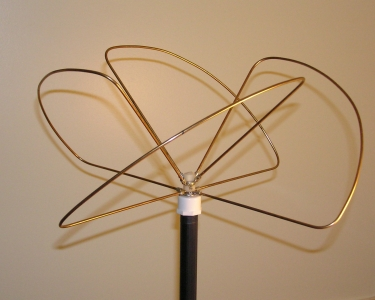
\includegraphics[width=0.5\linewidth]{Planar.jpg}
	\caption{Kleeblattantenne mit vier Bögen \cite{website}.}\label{fig:Planar}
\end{figure} 

Abbildung \ref{fig:Planar} zeigt dabei eine Kleeblattantenne mit vier Bögen, welche für die Simulation modelliert wurde.

\subsection{Theorie}

Um die Antenne aufbauen zu können sind folgende Berechnungen durchgeführt worden:\\

\begin{figure}[!ht]
	\centering
	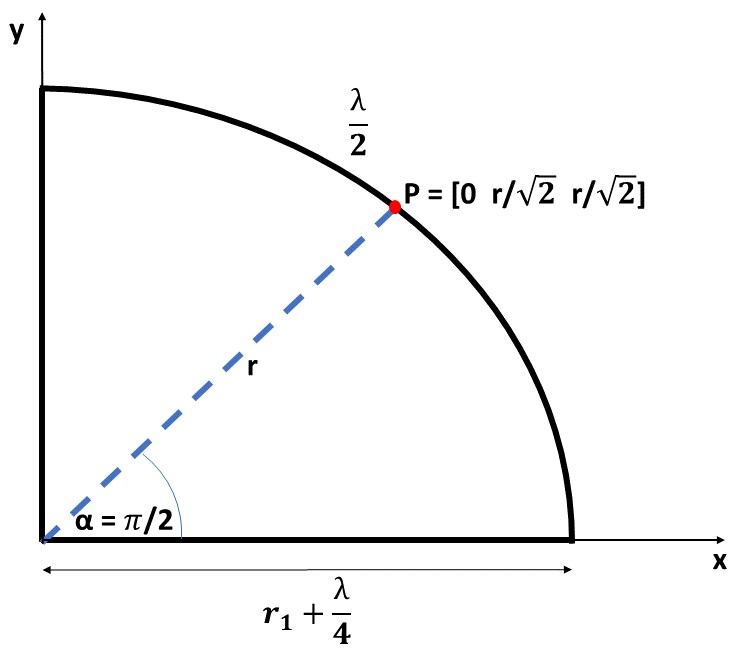
\includegraphics[width=0.5\linewidth]{berechnung}
	\caption{Aufbau eines Kleeblattbogens.}\label{fig:berechnung}
\end{figure}

In der Abbildung \ref*{fig:berechnung} ist ein Kleeblattbogen abgebildet. Die Länge $ r $ lässt sich als $ \lambda/4 + r_1 $ definieren. Der Bogen selber hat eine Länge von $\lambda/2$, wobei sich eine Länge von $\lambda + 2r_1$ für ein einzelnes Blatt einstellt. $r_1$ stellt den Radius des Vakuums in der Mitte dar, damit die effektive Länge des Bogens auch $\lambda$ beträgt, wenn ein Port zur Anregung angeschlossen wird. Der Punkt P gilt als Stützstelle für den Bogen, welcher durch die 3D Spline des Programmes angenähert wird.

\begin{figure}[!ht]
	\centering
	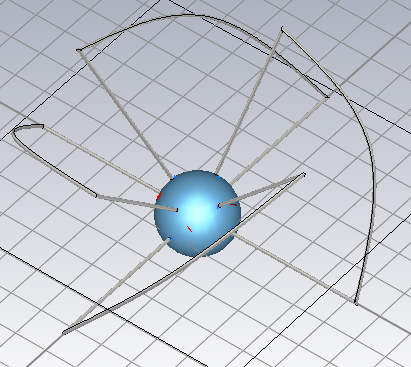
\includegraphics[width=\linewidth]{Kleeblatt}
	\caption{Modellierte Kleeblattantenne in CST.}\label{fig:Kleeblatt}
\end{figure}

Abbildung \ref{fig:Kleeblatt} zeigt die modellierte Kleeblattantenne. Mit dieser wurden die Simulationen durchgeführt.

\subsection{Simulation}

Für die Kleeblattantenne wäre eine Simulation vorgesehen gewesen. Jedoch konnte bisher keine erfolgreiche Simulation durchgeführt werden, da der Solver entweder frühzeitig abbricht, die Simulation nach mehreren Stunden nicht annähernd fertiggestellt werden konnte oder sogar der Prozessor abstürzte. Daher werden zur Abgabe dieses Projektes die Simulationsdateien beigefügt, damit nachträglich noch Simulationen durchgeführt werden können.